\documentclass{article}[11pt]
\textheight 8.5in
\usepackage{graphicx}
\usepackage{float}%for forcing position of figs
\usepackage{hyperref}
\usepackage{url}
\usepackage{amsmath}
\usepackage{amssymb}

\begin{document}
\begin{center}
Solving Multi-agent IRL using EM
\end{center}

\section{Summary of Discussions}
In this report we will discuss about Kantorovich metric and how it is used  as a bisimulation metrics in MDPs for knowledge transfer



\section{Kantorovich Metric}

Consider the transportation problem of transporting goods from one place to another through a network of roads. The Kantorovich metric is finding the most cost efficient way of transporting goods given a cost of transport from one node to another. In probability distributions, this can be interpreted as the total cost of transforming one probability distribution to another under a given given a distance metric to transport each quantum of probability.

Let $\mathcal{M}$ be the space of bounded distance metrics on the set $\mathcal{X}$ and let $\mathcal{M}_P$ be the space of probability distribution metrics for distributions on $\mathcal{X}$. The Kantorovich metric, $T_K : \mathcal{M} \to \mathcal{M}_P$ is defined by the following primal linear program for $\mu, \nu \in \mathcal{P}(\mathcal{X})$

\begin{align*}
&T_K(d) (\mu,\nu) = \max_x \sum_{s \in S} (\mu(s) - \nu(s))x_s\\
&\text{s.t.   } x_s-x_{s'} \le d(s,s') \ \ \forall s,s' \in S\\
&\ \ \ \ \ \ \ \ \ \ \ \ \ x_s \ge 0 \ \ \forall s \in S
\end{align*}

The dual of this problem is given by,
\begin{align*}
&\min_\lambda \sum_{s \in S}\sum_{t \in S} \lambda_{s,t}d(s,t)\\
\text{s.t.} & \sum_{t\in S}\lambda_{s,t} = \mu(s) \ \ \forall s \in S\\
& \sum_{s\in S}\lambda_{s,t} = \nu(s) \ \ \forall t \in S\\
&\lambda_{s,t} = \ge 0 \ \ \forall s,t \in S
\end{align*}

This can be intuitively interpreted as a network flow problem. Assume we have a source node denoted by $src$ and sink node $snk$. Our aim to move all data from source to sink through two layers of states. The second laer is a copy of the first layer. Edge from $src$ to each state $s$ in the first layer has a capacity of $\mu(s)$ and similarly edge from each state $t$ in the second layer to $snk$ has a capacity of $\nu(t)$. The states in the first and the second layer are fully connected and have infinite capacity but come with a cost $d(s,t)$. The problem then is to find the mass of data through each edge to got from $src$ to $snk$

\begin{figure}[H]
  \begin{center}
    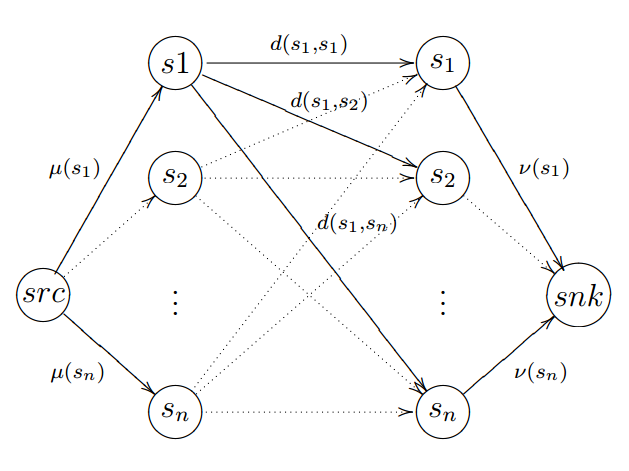
\includegraphics[width=0.7\linewidth]{images/network.png}
    \caption{Kantorovich metric as a network traffic problem. Image from \cite{castro2011planning}}
    \label{fig:cem}
  \end{center}
\end{figure}

\section{Bisimulation Metric}
Using exact equivalence of two states to compute similarity may make two equivalent state no longer equivalent even under small perturbations of reward and transition probabilities. 

Consider the difference in optimal value functions \cite{ferns2004metrics}
\begin{align*}
|V^*(s) - V^*(t)| \le \max_{a \in A} (|r^a_s-r^a_{t}| + \gamma |\sum_u(P^a_{su} - P^a_{tu})V^*(u)|)
\end{align*}

Note that the second component of RHS resembles the dual Kantorovich metric LP. Based on this, if we define 

\begin{align*}
F(d)(s,s') = \max_{a\in A}(|R(s,a) - R(t,a)| + \gamma T_K(d)(P(s,a),P(t,a)))
\end{align*}

\cite{ferns2004metrics} proves that $F$ has a greatest fixed point $d_{\sim}$ and $d_{\sim}$ is a bisimulation metric.

Also, \cite{castro2011planning} states that $|V^*(s) - V^*(t)| \le d_{\sim}(s,t)$ (Proof in page 111). The nice thing about this is that the states $s$ and $t$ need not be in the same MDP. This is where  Kantorovich metric is mainly advantageous since it gives a distance between probability distributions on different spaces as long as a distance metric $d$ is defined between them. Hence, we can transfer the values from one state to another if $d_{\sim}(s,t) \le \delta$


\section{Plans for effiecient computation of  Kantorovich metric}
As we saw that in the review paper, they used the nominal distribution $\nu(s)$ with finite support. Here the problem becomes similar if we assume that the target state to transfer to has finite support. In \cite{castro2011planning}, however, they use empirical estimates of the transition probability distributions of source and target to compute Kantorovich metric efficiently. Importantly, the main contribution of the review paper was to solve the min-max bellman equation efficiently using Kantorovich metric. In Kantorovich metric, they are concerned about computing the Kantorovich metric itself more efficiently. However, I am still interested in exploring if finite support assumption makes empirical  Kantorovich metric computation in Kantorovich metric more efficient.


\section{Bibliography}

\bibliographystyle{plain}
\bibliography{bibfile}
\end{document}
